\section{Systemsekvens Diagram}
\begin{figure}[!ht]
\centering
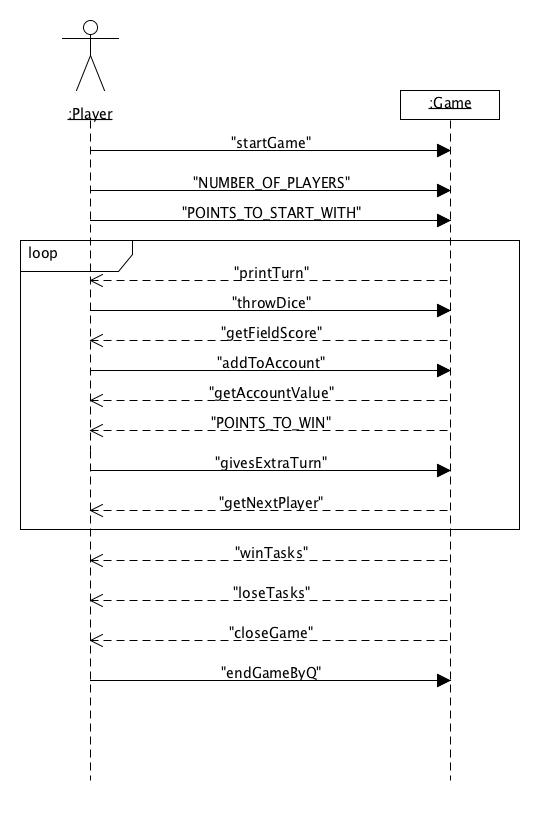
\includegraphics[scale=0.4]{SystemSequenceDiagramDieGame.jpg}
\caption[<Text for the list of figures>]{Systemsekvens Diagram}
\label{fig:figure 2} 
\end{figure}
Vores System sekvens diagram tager udgangspunkt i vores fully dressed use case: spil. Det første der sker, er at selve spillet startes. Herefter finder vi ud af hvor mange spillere, der er. Spillernes startbalance bliver nu sat. Herefter vil spillet kører i en løkke, indtil en af spillerne har tabt eller vundet. Løkken printer turen på spilleren. Terningen kastes. Spilleren får konsekvensen af det felt han lander på. Beløbet bliver overført til spillerens konto. Spilleren får nu vist hvad balancen er på kontoen. Der bliver kontrolleret, hvor vidt spilleren har opnået point nok til at vinde eller har mistet alle sine penge (Her mangler en metode til at kontrollere balancen på spillerens konto). Hvis det er tilfældet hopper vi ud af løkken. Hvis det er et bestemt felt på pladen, skal spillet give spilleren en ekstratur (Pilen vender den forkerte vej i diagrammet). Dette vil give ham en tur mere i løkken. Hvis ingen af disse ting forekommer, giver spillet turen videre. Hvis en spiller har vundet, skriver konsollen, hvilken spiller det er og hans point. Hvis en spiller har tabt, skriver konsollen, hvilken spiller der så har vundet og hans point. Efter det lukker spillet. Spilleren har hele tiden mulighed for at stoppe spillet med tasten "q".
\\
Systemsekvensdiagrammet er vigtigt at have med, da det vise hvordan systemet reagere på udefrakommende inputs. Det giver også indblik i hvordan systemet skal fungere uden at skulle skrive en masse kode.